\documentclass{article} % For LaTeX2e
\usepackage{nips13submit_e,times}
\usepackage{hyperref}
\usepackage{epsfig}
%\usepackage{mahnig}
\usepackage{url}
\usepackage{enumerate}
\usepackage{booktabs}
%\documentstyle[nips13submit_09,times,art10]{article} % For LaTeX 2.09
\usepackage{multicol}

\usepackage{graphicx} 
\graphicspath{ {./images/} }

\title{Automatic Image Caption Generation}

\author{Oihane Cantero and Julen Etxaniz}

% The \author macro works with any number of authors. There are two commands
% used to separate the names and addresses of multiple authors: \And and \AND.
%
% Using \And between authors leaves it to \LaTeX{} to determine where to break
% the lines. Using \AND forces a linebreak at that point. So, if \LaTeX{}
% puts 3 of 4 authors names on the first line, and the last on the second
% line, try using \AND instead of \And before the third author name.

\newcommand{\fix}{\marginpar{FIX}}
\newcommand{\new}{\marginpar{NEW}}

\nipsfinalcopy % Uncomment for camera-ready version

\begin{document}

\maketitle

\begin{abstract}

Automatic image caption generation is an attractive and challenging machine learning task. It can be useful for visual impaired people, to allow them to have a clear description of an image. It combines both computer vision and natural language processing, and it can be difficult to make descriptions that are correctly made and describe the scene of the image the most precisely possible. In this report, we will show which different models we have implemented, and the results we obtained.

\end{abstract}

\tableofcontents

\newpage

\section{Introduction} \label{intro}

Automatic image caption generation consist on automatically create captions of images, not to have to create them manually. It can be very helpful for people suffering from visual impairment, or simply to create captions when we have large datasets and we have to describe the images.
In this project we will build a deep learning model that generates descriptions of given photograph. The project requires to combine different deep learning architectures such as CNNs and LSTMs. Implemented model will be evaluated according to the BLEU standard metric used in the field.

These are the objectives of the project:

\begin{itemize}
    \item Implement from scratch a caption generation model that uses a CNN to condition a LSTM based language model \cite{ShowTell}. 
    \item Extend the basic caption generation system that incorporates an attention mechanism to the model \cite{ShowAttendTell}. 
\end{itemize}

\section{Approach}

We decided to start with the simplest approach and add more complexity if we had time. So, we started with the model without attention and with the Flickr8k dataset introduced in \cite{Flickr8k}. It can be downloaded from \url{https://github.com/jbrownlee/Datasets/releases/tag/Flickr8k}. We thought that we could change to Flickr-30k dataset if we wanted a bigger one: \url{http://bryanplummer.com/Flickr30kEntities/}.

We decided to work with Google Colaboratory because it offers access to GPUs for free. We also thought about using Kaggle, because it offers a similar environment. We also found out that the datasets we needed were also available there: \url{https://www.kaggle.com/shadabhussain/flickr8k} and \url{https://www.kaggle.com/hsankesara/flickr-image-dataset}. So, we wouldn't have to download them. At the end, we decided to go on with Colab because it was easier to work with files from Google Drive.

In general, it was a good experience, but we reached the usage limits several times. We had Google Drive syncronized so that we could make changes in both places without needing to upload and download files. We also created a \href{https://github.com/juletx/neural-caption-generation}{GitHub repository} and commited the code when there were some improvements to keep track of changes and have backups. The Jupyter Notebook at GitHub can also be accessed from \href{https://colab.research.google.com/github/juletx/neural-caption-generation/blob/main/notebook/P71_OIER_Caption_Generation.ipynb}{Colab}.

\subsection{No Attention}
Firstly, we read the paper about image captioning without attention: \cite{ShowTell}. Then, we had a look at some tutorials about image captioning: \url{https://machinelearningmastery.com/develop-a-deep-learning-caption-generation-model-in-python/}. 

We also had a look at \url{https://paperswithcode.com/paper/show-and-tell-a-neural-image-caption} to find more implementations. We found some that there were useful examples such as \url{https://github.com/yashk2810/Image-Captioning} and \url{https://github.com/dabasajay/Image-Caption-Generator}.

We run and experimented with the tutorials and examples ourselves to understand how they were working. Next, we started implementing our notebook \texttt{P71\_Caption\_Generation.ipynb}.

We tested different models and we obtained decent metrics and captions in general. So, we decided to try implementing the attention mechanism.

\subsection{Attention}

Firstly, we read the paper about image captioning with attention: \cite{ShowAttendTell}. Then, we had a look at some tutorials: \url{https://www.tensorflow.org/tutorials/text/image_captioning},  \url{https://medium.com/swlh/image-captioning-using-attention-mechanism-f3d7fc96eb0e} and \url{https://www.analyticsvidhya.com/blog/2020/11/attention-mechanism-for-caption-generation/}.

The tutorials we found were mostly implemented with tensorflow. It seemed that it was necessary to implement the models on a lower level to implement attention correctly and plot the images.

As we had done our implementation with keras this required changing many things. We tried adding an attention layer to the keras model but we didn't achieve any improvements. We also did not know how to plot the attention. 

So, we decided to create a new notebook \texttt{P71\_Caption\_Generation\_Attention.ipynb} and start implementing the attention model with tensorflow. When we had a minimum version that was generating quite good captions, we started making some improvements. 

We implemented a validation step to measure the performance while it was training. We evaluated the model with BLEU. At some point, we broke something and the model and it stopped working correctly. We tried fixing it but we ran out of time, so the generated captions are very poor and the BLEU scores reflect that.

\section{Implementation}

We decided to separate the two tasks mentioned in Section \ref{intro} into two different notebooks to make them easier to follow: \texttt{P71\_Caption\_Generation.ipynb} and \texttt{P71\_Caption\_Generation\_Attention.ipynb}. They have some parts in common and some other are different. So, we have made subsections to separate them when they are different.

On the one hand, the datasets, the preparation of the text data, the way we load it is the same. The way we encode data is similar. On the other hand, the way extract photo data changes. The defined model and the fit strategy change a lot.

\subsection{Get Dataset}

We decide to use the Flickr8k dataset introduced in \cite{Flickr8k}. It has 8092 images and 5 captions for each image. Each image has 5 captions because there are different ways to caption an image. This dataset has predefined training, testing and evaluation subsets of 6000, 1000 and 1000 images respectively.

\subsection{Prepare Photo Data}

\subsubsection{No Attention}
We use two pretrained CNN models to extract features from images: VGG16 and InceptionV3. See Figures \ref{VGG16} and \ref{InceptionV3}. We remove the last layers of these models because we are not interested in classifying images. We are interested in the representation of the images.
Instead of extracting the features every time we need them, we compute all of them and save to a file. We saved the features extracted with each model in a different file: \texttt{features\_vgg16.pkl} and \texttt{features\_inceptionv3.pkl}.

These models require images of a concrete size, 224 and 299 pixels respectively. So, images had to be resized, then converted to array and reshaped. The extracted features are vectors of size 4096 and 2048.

\begin{figure}[ht]
\centering
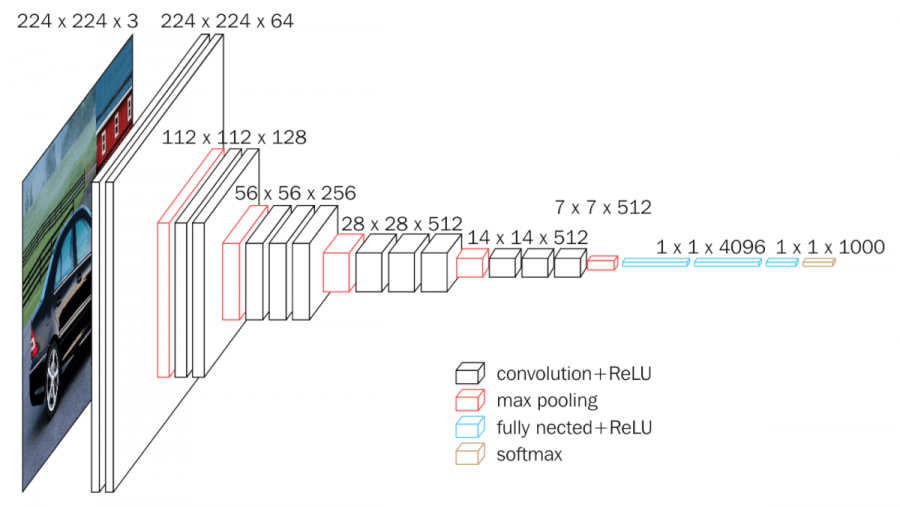
\includegraphics[width=\textwidth]{vgg16.png}
\caption{VGG16 model} 
\label{VGG16}
\end{figure}

\begin{figure}[ht]
\centering
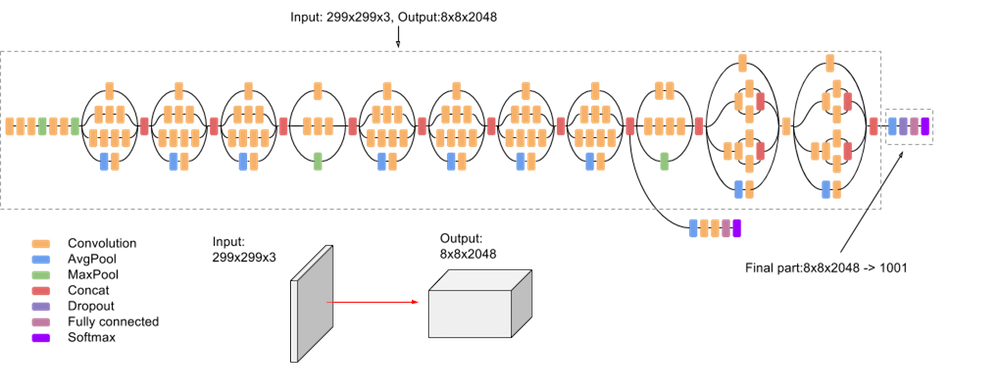
\includegraphics[width=\textwidth]{inceptionv3.png}
\caption{InceptionV3 model} 
\label{InceptionV3}
\end{figure}

\subsubsection{Attention}
In the notebook with attention, we only used VGG16, but not exactly the same dimensions. We use the layer with dimension 7x7x512 to extract features from images. Instead of saving all the features in the same file, we dump them to a numpy file with the same name of the images so that we can use them later. Each file has 98KB.

We also tried with InceptionV3, but the generated numpy files were too big, 512KB each. That is because the shape of the extracted features is 8x8x2048, much bigger than with VGG16.

\subsection{Prepare Text Data}

Firstly, we load all the descriptions of the images. We create a dictionary that maps image names to descriptions. To prepare the text data, we needed to clean the description of the images. For this, we converted all the words to lowercase, we removed all the punctuation, words one character long and words with numbers. 

Next, we create a vocabulary with the unique words of the descriptions. The size of the created vocabulary is 8,763. Finally, we save the descriptions to the file \texttt{descriptions.txt} so that we can use them later.

\subsection{Load Data}

We define functions to load data that correspond to each of the subsets: train, validation and test. These subsets are predefined in files: \texttt{Flickr\_8k.trainImages.txt}, \texttt{Flickr\_8k.devImages.txt} and \texttt{Flickr\_8k.testImages.txt}. In the notebook without attention we load the image keys, descriptions and features. In the case of attention we don't load features because we extract them later.

The model will generate a caption word by word taking into account the previous words. So, we need initial and final word to start and end the generation. That's why we added \texttt{<start>} and \texttt{<end>} to the descriptions as initial and final word.

\subsection{Encode Text Data}

Here we use a tokenizer to create a map from words of the vocabulary to integers. We save this tokenizer at the file \texttt{tokenizer.pkl} to use it later. We also calculate the size of the vocabulary and the maximum length of descriptions to use them later.

In the case of attention, We limited the vocabulary size to the 5000 most common words. Therefore, we put \texttt{<unk>} token to all the words that are not in the vocabulary. Moreover, if the caption is shorter that the maximum length we make a padding that adds \texttt{<pad>} token. We saved this tokenizer to \texttt{tokenizer2.pkl}. We used it to convert all the descriptions to integers.

\subsection{Define Model}

As we have seen before, the project has two objectives, and here, we have implemented three models, two without using attention and one with attention. 

\subsubsection{No Attention}

We decided to try different Recurrent Neural Network architectures and compare the results. As we can see in figures \ref{Model1} and \ref{Model2}, the models are different, but both have a Long Short-Term Memory network as recursive network. See Figures \ref{Model1} and \ref{Model2}.

\begin{figure}[ht]
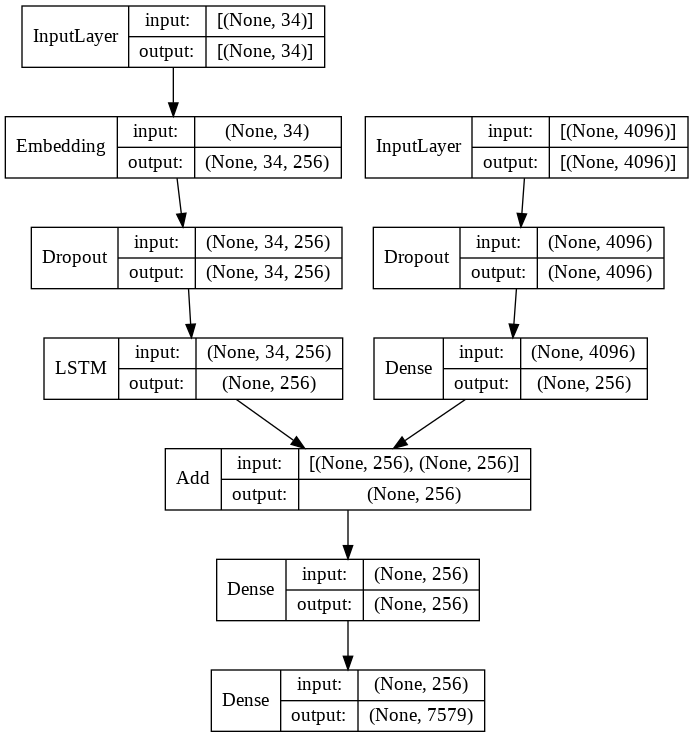
\includegraphics[width=\textwidth]{rnn_model_1_vgg16.png}
\caption{Model 1: It has two inputs. In the text submodel it has an Embedding, Dropout and LSTM layers. In the image submodel, it has a Dropout and a Dense layer. Then it adds these two submodels and finally there are two Dense layers, the last one having vocabulary size with softmax.}
\label{Model1}
\end{figure}

\begin{figure}[ht]
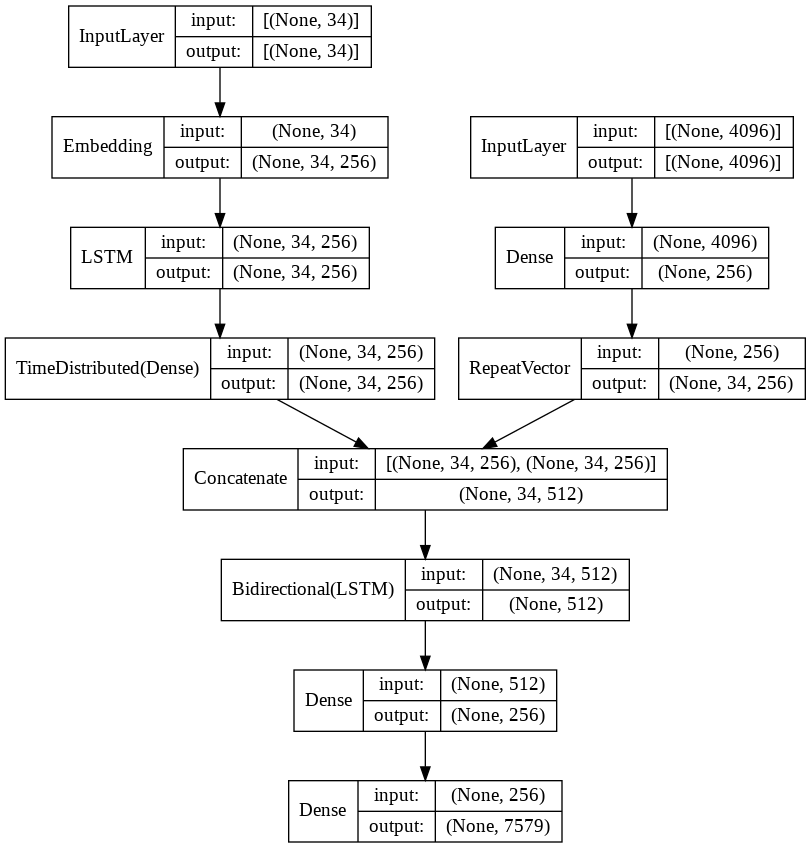
\includegraphics[width=\textwidth]{rnn_model_2_vgg16.png}
\caption{Model 2: It has two inputs. In the text submodel it has an Embedding, LSTM and TimeDistributed Dense layers. In the image submodel, it has a Dense and a RepeatVector layer. Then it concatenates these two submodels. finally there are two Dense layers, the last one having vocabulary size with softmax.}
\label{Model2}
\end{figure}

\subsubsection{Attention}

We decided to implement Local attention, using Bahdanau's implementation, also known as Additive Attention, which only implements attention in a few input sources.

Since you have already extracted the features, the encoder part of the model is composed of an unique dense layer. The attention is implemented in the Decoder part of the model. The decoder is composed of an embedding layer, a LSTM layer, two dense layers separated by a dropout and a batch normalization layer and an attention layer. The dropout is done with a probability of $0.5$ and together with the batch normalization layer, they help to avoid overfitting.

\subsection{Fit Model}

\subsubsection{No Attention}

In this part, we fit the model to the data we had. We monitor training and validation loss. We save the best the model with lowest validation loss in order to use it later, because fitting can be very long. If the validation loss increases in two consecutive epochs we stop training to save time and avoid overfitting.

We tried all the possible combinations between the different CNN's with the RNN's and we can see in figure \ref{lossgraph} that the best result (regarding to the loss) without attention have been for the second RNN (see figure \ref{Model2}) and Inceptionv3 models. 

The model receives image features, a sequence of words and the output word. Instead of doing this with all the data we create these sequences for one image at a time. For each image and caption we create all the possible input sequences and output words by adding one word until we reach \texttt{<end>}.

We created a data generator for the training set and another one for the validation set.

We defined the maximum number of epochs to 20 and the batch size to 32. We calculated the number of steps needed in each epoch for training and validation data.

And we use a data generator to generate arrays of these sequence of the size of the batch progressively. We used this approach to avoid reaching RAM and GPU limits. Otherwise, we weren't able to train the model with the RAM available in Google Colaboratoty. The data generator receives the training data shuffled and works with image ids to take the images that correspond to the captions.

Finally, we visualize the training and validation loss to know better how our model is learning. See figure \ref{lossgraph}.

\begin{figure}[ht]
\centering
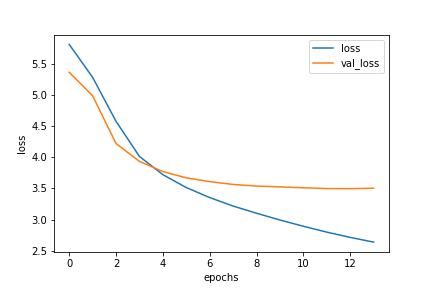
\includegraphics[scale=0.5]{rnn_2_inceptionv3_loss.png}
\caption{loss and val loss values on different epochs for RNN2 and Inceptionv3}
\label{lossgraph}
\end{figure}

\subsubsection{Attention}

In the model with attention, the idea is the same, we want to fit the model to our data, and save it in order to use it later, without having to train the model again.

We create train and validation datasets that are used to train the model. We define train and validation steps. We calculate the loss and validation loss after each epoch. If the validation loss decreases, we save the model weights.

We plot the training loss and validation losses. We can clearly see that the model is overfitting. See figure \ref{attlossgraph}.

\begin{figure}[ht]
\centering
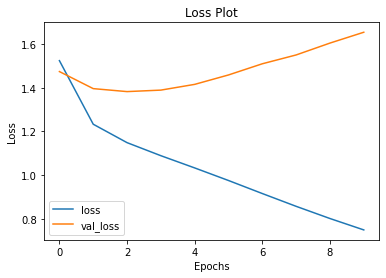
\includegraphics[scale=0.5]{attentionlosses.png}
\caption{loss and val loss values on different epochs for the model with attention}
\label{attlossgraph}
\end{figure}

\subsection{Evaluate Model}

We used two different ways to generate descriptions of images: Sampling and Beam search. Sampling consists of taking the best word at each time step until the end is reached. Beam Search considers the k best sentences at each time step. It predicts the next words for each one of them. Generally, making k bigger increases the chance of getting the description with the highest probability. 

But, it also increases the time needed to generate captions. We tried to evaluate with beam search the whole test set but took too long. So, we only used the Beam Search function to generate captions. 

Taking into account that we have created multiple models, we needed to find an effective way to evaluate the models. So, we choose to calculate the BLEU-scores on the test data to evaluate the models. This requires comparing the original captions with the generated ones.

\subsubsection{No Attention}
The BLEU scores we got from sampling, in the models without attention were these ones.

\begin{itemize}
\begin{multicols}{2}
    \item Sampling Model 1 VGG16
    \item BLEU-1: 54.114390
    \item BLEU-2: 33.489586
    \item BLEU-3: 24.785442
    \item BLEU-4: 13.031321
    \item Sampling Model 1 InceptionV3
    \item BLEU-1: 57.458612
    \item BLEU-2: 34.077377
    \item BLEU-3: 24.426512
    \item BLEU-4: 12.300981 
\end{multicols}
\end{itemize}

\begin{itemize}
\begin{multicols}{2}
    \item Sampling Model 2 VGG16
    \item BLEU-1: 59.5796
    \item BLEU-2: 36.9997
    \item BLEU-3: 27.2431
    \item BLEU-4: 14.4684
    \item Sampling Model 2 InceptionV3
    \item BLEU-1: 58.7866
    \item BLEU-2: 36.6849
    \item BLEU-3: 27.0134
    \item BLEU-4: 14.4244
\end{multicols}
\end{itemize}

As we can see, we obtained the best results using VGG 16 and the second model. After that comes Inceptionv3 and the second model. So we can conclude that the second RNN model was better than the first.

\subsubsection{Attention}
And the scores of the model with attention were the following ones. We can see that the scores are very bad compared to the model with no attention. This has a clear impact in the generated captions.

\begin{itemize}
    \item Sampling
    \item BLEU-1: 35.898466
    \item BLEU-2: 14.188016
    \item BLEU-3: 7.816680
    \item BLEU-4: 2.461979
\end{itemize}


\subsection{Generate Captions}

\subsubsection{No Attention}
We generate captions for some images of the test set to view the performance of our models with real examples. We used the same methods that were used for evaluation. But, instead of printing them as they are, we clean them to improve readability. This is done by removing the <start> and <end> words, and removing all the other tokens also.

For each image, we show the 5 original captions, the result of the sampling, and the result of beam search when k=3 and k=5. We also show BLEU-1 scores as reference for all the generated captions.

On the one hand, the captions generated without attention are quite good. They have some mistakes but they capture some aspects of the images correctly. On the other hand, the captions are very bad with the attention model. This correlates with the low BLEU scores.

These are some results we had with some images from the test dataset, using Inceptionv3 and the second RNN model. We put one of the best and worst results to compare.


\begin{figure}[ht]
\centering
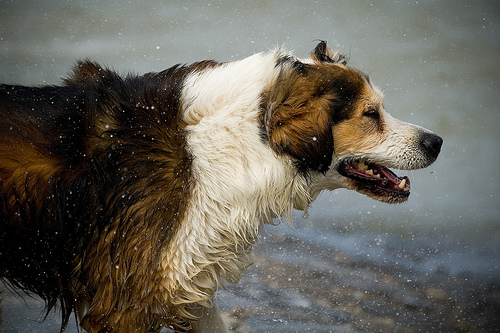
\includegraphics[scale=1]{dog.jpeg}
\caption{One of the best captioning\newline
Original 1: brown and white dog stands outside while it snows\newline
Original 2: dog is looking at something near the water\newline
Original 3: furry dog attempts to dry itself by shaking the water off its coat\newline
Original 4: white and brown dog shaking its self dry\newline
Original 5: the large brown and white dog shakes off water\newline
Sampling (BLEU-1: 58.4101): dog is swimming in the water\newline
Beam Search k=3 (BLEU-1: 72.7273): white and white dog is swimming in the water\newline
Beam Search k=5 (BLEU-1: 70.0000): brown and white dog swims in shallow water\newline}
\label{dog}
\end{figure}


\begin{figure}[ht]
\centering
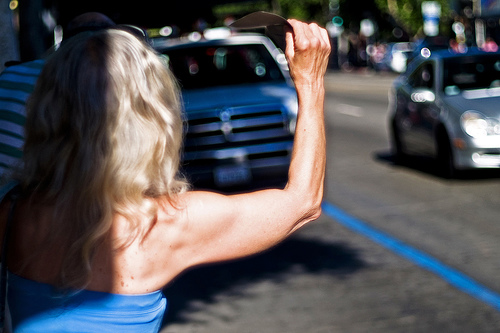
\includegraphics[scale=1]{womanstreet.jpeg}
\caption{One of the worst captioning\newline
Original 1: blond woman in blue shirt appears to wait for ride\newline
Original 2: blond woman is on the street hailing taxi\newline
Original 3: woman is signaling is to traffic as seen from behind\newline
Original 4: woman with blonde hair wearing blue tube top is waving on the side of the street\newline
Original 5: the woman in the blue dress is holding out her arm at oncoming traffic\newline
Sampling (BLEU-1: 50.0000): the boy is wearing red hat and is wearing helmet\newline
Beam Search k=3 (BLEU-1: 60.0000): the boy is wearing red shirt and helmet \newline
Beam Search k=5 (BLEU-1: 50.0000): young boy wearing helmet and blue shirt is wearing helmet}
\label{womanstreet}
\end{figure}


While training, we have seen that we had the best results with Inceptionv3 and the 2nd RNN model. But there is a lot of improvement to do yet, as we can see in the Figure \ref{womanstreet} captioning, for example. Also, in figure \ref{dog}, we can see that there is still work to do, because, even if we have a quite correct description, it is not very close from any of the original ones.

\subsubsection{Attention}

Here, we can see which have been our results for the same images using the model with attention. Although, we can see where the attention was "focusing" at each step. 

\begin{figure}[ht]
\centering
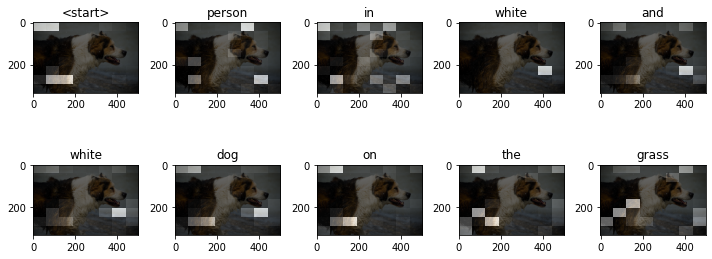
\includegraphics[scale=0.5]{attentiondog.png}
\caption{One of the captioning with attention\newline
Original 1: brown and white dog stands outside while it snows\newline
Original 2: dog is looking at something near the water\newline
Original 3: furry dog attempts to dry itself by shaking the water off its coat\newline
Original 4: white and brown dog shaking its self dry\newline
Original 5: the large brown and white dog shakes off water\newline
Sampling (BLEU-1: 54.545455): person in white and white dog on the grass\newline}
\label{attdog}
\end{figure}

\begin{figure}[ht]
\centering
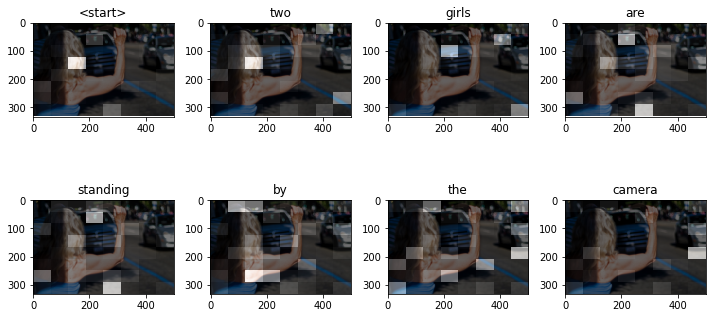
\includegraphics[scale=0.5]{attentionwoman.png}
\caption{One of the captioning with attention\newline
Original 1: blond woman in blue shirt appears to wait for ride\newline
Original 2: blond woman is on the street hailing taxi\newline
Original 3: woman is signaling is to traffic as seen from behind\newline
Original 4: woman with blonde hair wearing blue tube top is waving on the side of the street\newline
Original 5: the woman in the blue dress is holding out her arm at oncoming traffic\newline
Sampling (BLEU-1: 29.827977): two girls are standing by the camera\newline}
\label{attwomanstreet}
\end{figure}

As we can see, our results with attention are worst than the results without. We managed to understand why, and we think it can be an implementation problem. But we didn't have enough time to find where was the error.

\section{Conclusion}

Generating captions for images is a difficult task. Most of the times there were some mistakes in the captions. Comparing it to the scores of the referenced papers we get a lower score. But, we could say that it is still a decent score. We also tried to implement attention but it has been in vain, because the results where worst than those without attention.

In conclusion, we have seen that even if we trained several models, we have approximately the same results. As improvements, we have thought about generating captions using Beam Search, using bigger datasets, and succeeding implementing attention. We could also use pretrained word embeddings. Finding a better model architecture could also improve the scores.

\bibliographystyle{unsrt}
\bibliography{bibtex_references_project}

\end{document}
